\documentclass[a4paper,11pt]{article}
\usepackage[T1]{fontenc}
\usepackage[utf8]{inputenc}
\usepackage{lmodern}
\usepackage{upgreek}
\usepackage{amsmath}
\usepackage[]{algorithm2e}
\usepackage{hyperref}
\usepackage{tikz}
\usetikzlibrary{automata,positioning}

\title{Programovací jazyk SVGER}

\begin{document}

\maketitle
\newpage
\tableofcontents

\newpage
\section{Gramatiky a lexikální analyzátor}
Programovací jazyk se skládá z následujících gramatik:
$Q_{f}$
\subsection{Identifikátory}
Identifikátor začíná na kterýkoliv znak z množiny $z = \{a..z,A..Z,+,-/,*,<,>,[,]\}$
a pokračuje v kterémkoliv ze znaků z množiny $m = z \bigcup \{0..9\}$ 
\linebreak

Z tohoto popisu nám vyplyne následující gramatika $L_\{identifikatory\}$(['S', "S'"], ['z', 'm'], \{
$$S \rightarrow zS|z|S'$$$$S' \rightarrow mS'|m$$\},
S)

\subsubsection{Nalezení symbolů, které nejsou zbytečné}$$\uptau_0 = \{m,z\}$$$$\uptau_1 = \{S,S',m,z\}$$\subsubsection{Hledání dostupných symbolů}$$D_0 = \{S\}$$$$D_1 = \{S,S',z\}$$$$D_2 = \{S,S',m,z\}$$\subsubsection{Upravená gramatika}
Po úpravách dostaváme gramatiku
$L_\{identifikatory\}$(['S', "S'"], ['z', 'm'], \{
$$S \rightarrow zS|z|S'$$$$S' \rightarrow mS'|m$$\},
S)

\subsubsection{Generování automatu}
Stavy automatu \{$Q_{S}$,$Q_{S'}$,$Q_{F}$\}
\subsubsection{Tabulka}
\begin{center}
\begin{tabular}{c c c }
& z& m
S
&z
&S
&z
&S'
S'
&m
&S'
&m
\end{tabular}
\end{center}


\subsection{Čísla}
Jazyk obsauje pouze přirozená čísla. Validním číslem je tedy jakákoliv sekvence znaků, které se nachází v množině $d = {0..9}$

Ná základě tohoto můžeme vytvořit následující gramatiku $L_cisla$(['S', 'A', 'B', 'C'], ['-', 'd', '.'], \{
$$S \rightarrow -A|dA|d|dC$$$$A \rightarrow dA|d|dC$$$$B \rightarrow dB|d$$$$C \rightarrow .B$$\},
S)

\subsubsection{Nalezení symbolů, které nejsou zbytečné}$$\uptau_0 = \{-,.,d\}$$$$\uptau_1 = \{-,.,A,B,C,S,d\}$$\subsubsection{Hledání dostupných symbolů}$$D_0 = \{S\}$$$$D_1 = \{-,A,C,S,d\}$$$$D_2 = \{-,.,A,B,C,S,d\}$$\subsubsection{Upravená gramatika}
Po úpravách dostaváme gramatiku
$L_cisla$(['S', 'A', 'B', 'C'], ['-', 'd', '.'], \{
$$S \rightarrow -A|dA|d|dC$$$$A \rightarrow dA|d|dC$$$$B \rightarrow dB|d$$$$C \rightarrow .B$$\},
S)

\subsubsection{Generování automatu}
Stavy automatu \{$Q_{S}$,$Q_{A}$,$Q_{B}$,$Q_{C}$,$Q_{F}$\}


\subsection{Slova}
$L_slova$(SABC, ab, \{
$$S \rightarrow A|B$$$$A \rightarrow aB|AS|b$$$$B \rightarrow AB|bA|\epsilon$$$$C \rightarrow AS|b$$\},
S)

\subsubsection{Nalezení symbolů, které nejsou zbytečné}$$\uptau_0 = \{a,b\}$$$$\uptau_1 = \{A,B,C,a,b\}$$$$\uptau_2 = \{A,B,C,S,a,b\}$$\subsubsection{Hledání dostupných symbolů}$$D_0 = \{S\}$$$$D_1 = \{A,B,S\}$$$$D_2 = \{A,B,S,\epsilon,a,b\}$$\subsubsection{Upravená gramatika}
Po úpravách dostaváme gramatiku
$L_slova$(['S', 'A', 'B'], ['a', 'b'], \{
$$S \rightarrow A|B$$$$A \rightarrow aB|AS|b$$$$B \rightarrow AB|bA|\epsilon$$\},
S)

\subsubsection{Generování automatu}
Stavy automatu \{$Q_{S}$,$Q_{A}$,$Q_{B}$,$Q_{F}$\}


\subsection{Konečný automat}
\begin{center}
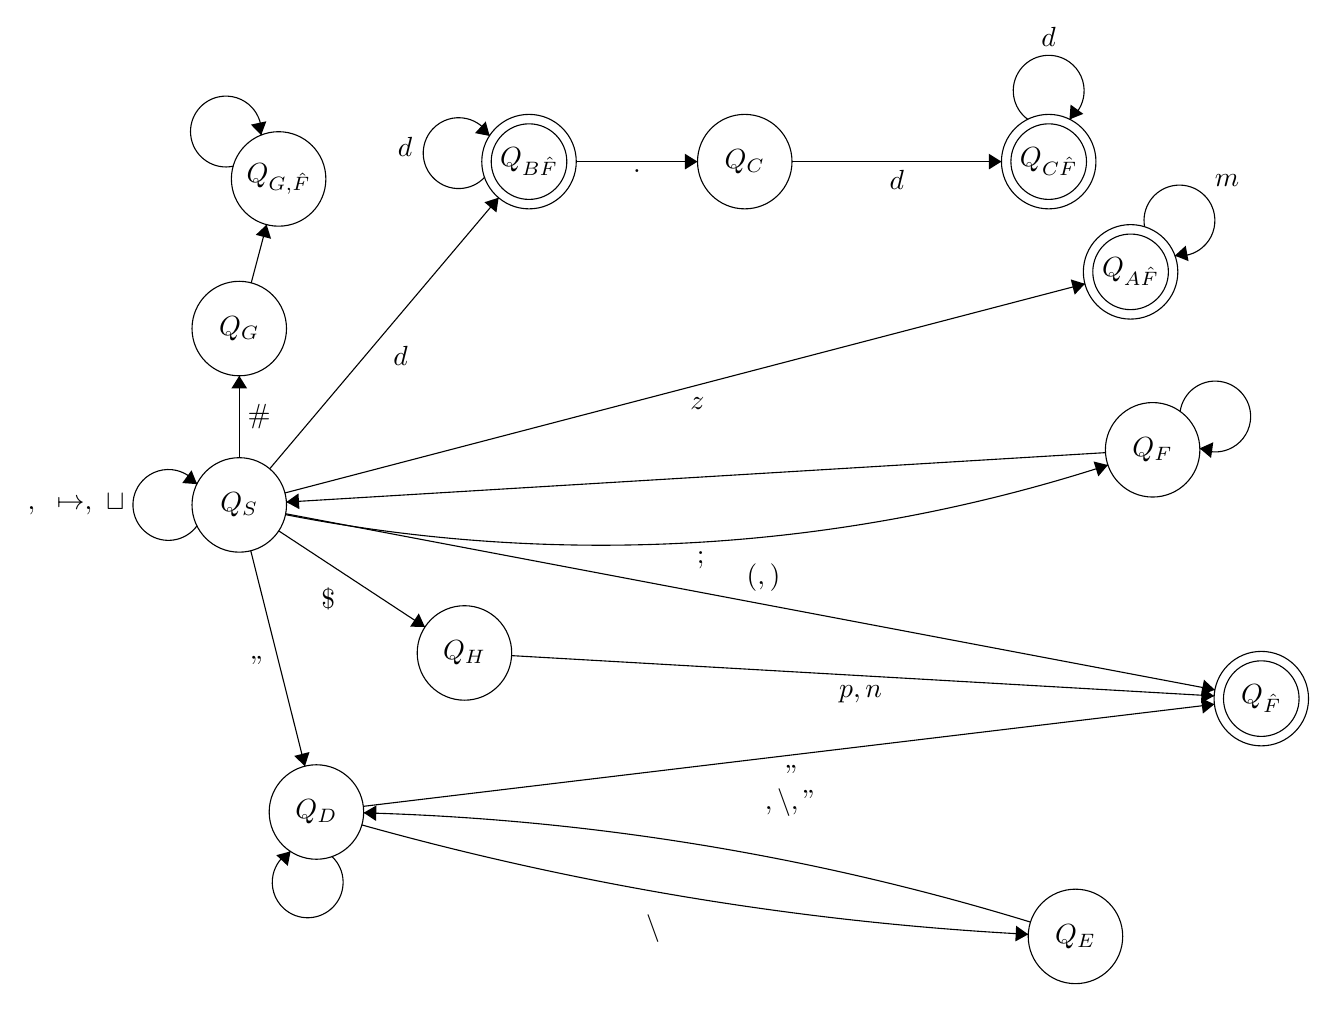
\begin{tikzpicture}[scale=0.2]
\tikzstyle{every node}+=[inner sep=0pt]
\draw [black] (8,-28.2) circle (3);
\draw (8,-28.2) node {$Q_{S}$};
\draw [black] (26.4,-6.4) circle (3);
\draw (26.4,-6.4) node {$Q_{B\hat{F}}$};
\draw [black] (26.4,-6.4) circle (2.4);
\draw [black] (64.6,-13.4) circle (3);
\draw (64.6,-13.4) node {$Q_{A\hat{F}}$};
\draw [black] (64.6,-13.4) circle (2.4);
\draw [black] (72.9,-40.5) circle (3);
\draw (72.9,-40.5) node {$Q_{\hat{F}}$};
\draw [black] (72.9,-40.5) circle (2.4);
\draw [black] (59.4,-6.4) circle (3);
\draw (59.4,-6.4) node {$Q_{C\hat{F}}$};
\draw [black] (59.4,-6.4) circle (2.4);
\draw [black] (12.9,-47.7) circle (3);
\draw (12.9,-47.7) node {$Q_{D}$};
\draw [black] (66,-24.7) circle (3);
\draw (66,-24.7) node {$Q_{F}$};
\draw [black] (61.1,-55.6) circle (3);
\draw (61.1,-55.6) node {$Q_{E}$};
\draw [black] (40.1,-6.4) circle (3);
\draw (40.1,-6.4) node {$Q_{C}$};
\draw [black] (22.3,-37.6) circle (3);
\draw (22.3,-37.6) node {$Q_{H}$};
\draw [black] (8,-17) circle (3);
\draw (8,-17) node {$Q_{G}$};
\draw [black] (10.5,-7.5) circle (3);
\draw (10.5,-7.5) node {$Q_{G,\hat{F}}$};
\draw [black] (9.93,-25.91) -- (24.47,-8.69);
\fill [black] (24.47,-8.69) -- (23.57,-8.98) -- (24.33,-9.63);
\draw (17.75,-18.74) node [right] {$d$};
\draw [black] (10.9,-27.44) -- (61.7,-14.16);
\fill [black] (61.7,-14.16) -- (60.8,-13.88) -- (61.05,-14.85);
\draw (37.09,-21.37) node [below] {$z$};
\draw [black] (10.95,-28.76) -- (69.95,-39.94);
\fill [black] (69.95,-39.94) -- (69.26,-39.3) -- (69.07,-40.28);
\draw (41.29,-33.71) node [above] {$(,)$};
\draw [black] (65.49,-10.547) arc (190.39718:-97.60282:2.25);
\draw (70.72,-8.03) node [above] {$m$};
\fill [black] (67.41,-12.37) -- (68.28,-12.72) -- (68.1,-11.74);
\draw [black] (58.077,-3.72) arc (234:-54:2.25);
\draw (59.4,0.85) node [above] {$d$};
\fill [black] (60.72,-3.72) -- (61.6,-3.37) -- (60.79,-2.78);
\draw [black] (8.73,-31.11) -- (12.17,-44.79);
\fill [black] (12.17,-44.79) -- (12.46,-43.89) -- (11.49,-44.14);
\draw (9.69,-38.41) node [left] {$"$};
\draw [black] (63.16,-25.667) arc (-72.01092:-101.08244:104.23);
\fill [black] (63.16,-25.67) -- (62.25,-25.44) -- (62.55,-26.39);
\draw (37.31,-31.12) node [below] {$;$};
\draw [black] (58.103,-55.466) arc (-93.00582:-105.61026:195.334);
\fill [black] (58.1,-55.47) -- (57.33,-54.92) -- (57.28,-55.92);
\draw (34.28,-54.21) node [below] {$\backslash$};
\draw [black] (15.88,-47.34) -- (69.92,-40.86);
\fill [black] (69.92,-40.86) -- (69.07,-40.46) -- (69.19,-41.45);
\draw (43.15,-44.68) node [below] {$"$};
\draw [black] (15.899,-47.753) arc (88.44043:72.94349:159.117);
\fill [black] (15.9,-47.75) -- (16.69,-48.27) -- (16.71,-47.28);
\draw (43.03,-48.03) node [above] {$\blacksquare,\backslash,"$};
\draw [black] (67.745,-22.274) arc (172.01431:-115.98569:2.25);
\draw (72.64,-20.37) node [right] {$\Square$};
\fill [black] (68.99,-24.61) -- (69.71,-25.22) -- (69.85,-24.22);
\draw [black] (5.32,-29.523) arc (-36:-324:2.25);
\draw (0.75,-28.2) node [left] {$\dlsh,\mbox{ }\mapsto,\mbox{ }\sqcup$};
\fill [black] (5.32,-26.88) -- (4.97,-26) -- (4.38,-26.81);
\draw [black] (63.01,-24.88) -- (10.99,-28.02);
\fill [black] (10.99,-28.02) -- (11.82,-28.47) -- (11.76,-27.47);
\draw (36.78,-25.79) node [above] {$\dlsh$};
\draw [black] (13.882,-50.522) arc (46.9079:-241.0921:2.25);
\draw (10.12,-55.53) node [below] {$\blacksquare$};
\fill [black] (11.26,-50.2) -- (10.35,-50.44) -- (11.08,-51.12);
\draw [black] (23.581,-7.392) arc (317.11154:29.11154:2.25);
\draw (19.03,-5.47) node [left] {$d$};
\fill [black] (23.9,-4.77) -- (23.65,-3.85) -- (22.97,-4.59);
\draw [black] (29.4,-6.4) -- (37.1,-6.4);
\fill [black] (37.1,-6.4) -- (36.3,-5.9) -- (36.3,-6.9);
\draw (33.25,-6.9) node [below] {$.$};
\draw [black] (43.1,-6.4) -- (56.4,-6.4);
\fill [black] (56.4,-6.4) -- (55.6,-5.9) -- (55.6,-6.9);
\draw (49.75,-6.9) node [below] {$d$};
\draw [black] (10.51,-29.85) -- (19.79,-35.95);
\fill [black] (19.79,-35.95) -- (19.4,-35.09) -- (18.85,-35.93);
\draw (13.65,-33.4) node [below] {$\$$};
\draw [black] (25.3,-37.77) -- (69.9,-40.33);
\fill [black] (69.9,-40.33) -- (69.13,-39.78) -- (69.08,-40.78);
\draw (47.46,-39.66) node [below] {$p,n$};
\draw [black] (8,-25.2) -- (8,-20);
\fill [black] (8,-20) -- (7.5,-20.8) -- (8.5,-20.8);
\draw (8.5,-22.6) node [right] {$\#$};
\draw [black] (8.76,-14.1) -- (9.74,-10.4);
\fill [black] (9.74,-10.4) -- (9.05,-11.05) -- (10.02,-11.3);
\draw (10.01,-12.75) node [right] {$\boxplus$};
\draw [black] (7.623,-6.69) arc (282.01279:-5.98721:2.25);
\draw (4.94,-1.53) node [left] {$\boxplus$};
\fill [black] (9.39,-4.72) -- (9.72,-3.84) -- (8.74,-4.05);
\end{tikzpicture}
\end{center}

\end{document}
